\chapter{Pixelové detektory radiace a vyčítací zařízení}	% + pro pixelové detektory
\label{kap:2}
Mezi možnosti detekovat ionizující záření patří mimo jiné, použití pixelových detektorů. Pomocí pixelových detektorů, konkrétněji hybridních pixelových detektorů, jsme schopni detailně změřit ionizující záření. V dalších částech této kapitoly bude popsána obecná činnost a princip detekce radiace pixelových detektorů. V části \ref{Timepix2}, bude konkrétně popsán detektor z rodiny Timepix \cite{Llopart}, detektor Timepix 2 \cite{tpx2_manual}. 

\section{Princip činnosti pixelových detektorů}
\label{kap:2.1}
V této části bude popsán obecný princip činnosti pixelových detektorů, který je společný pro detektory radiace z rodiny Timepix \cite{Llopart}, vyvíjenými pod záštitou CERN Medpipix Collaboration \cite{Medpix}. Pixelový detektor, přesněji hybridní pixelový detektor se skládá ze dvou oddělitelných částí, ze senzorové vrstvy a vrstvy s vyčítací elektronikou viz. obrázek \ref{fig:Timepix}. Právě toto rozdělení na senzorovou a vyčítací část označuje název hybridní detektor.
\par Senzorová vrstva je tvořena polovodičovým materiálem. Důležitými parametry senzorové vrstvy jsou typ polovodičového materiálu a její tloušťka. Nejčastěji používané materiály jsou $\text{Si}$, $\text{CdTe}$ a $\text{GaAs}$. Na senzorovou vrstvu je připojené vysoké napětí, označované jako \textit{bias voltage}. Toto vysoké napětí zajistí vyprázdnění oblasti v polovodičové struktuře senzorové vrstvy. Pokud částice ionizujícího záření interaguje v senzorové vrstvě, dojde k vytvoření náboje. Tento náboj je dále zpracován vyčítací elektronikou která je pomocí technologie nazývající se \textit{bump bond}, připojena k senzorové vrstvě.
\par Vyčítací vrstva (ASIC) je rozdělena na 256x256 individuálních pixelů. Každý pixel obsahuje potřebnou elektroniku ke zpracovaní náboje, vzniklého v senzorové vrstvě. Detailnější popis zpracování analogového náboje na úrovni jednotlivých pixelů, bude popsán pro konkrétní pixelový detektor Timepix 2 v části \ref{Timepix2}. Po analogovém zpracování signálu následuje digitální zpracování, poté je digitální signál převeden na výstupní plošky. Vyčítací vrstva je pomocí \textit{wire bond} technologie připojena k desce plošných spojů. Signály vedoucí z pixelových detektorů jsou následně zpracovány vyčítacím zařízením. Druhy vyčítacích zařízní budou popsány v části \ref{Vycitaci zarizeni}.
 \begin{figure}[h!]
 	\centering
 	\captionsetup{justification=centering}
 	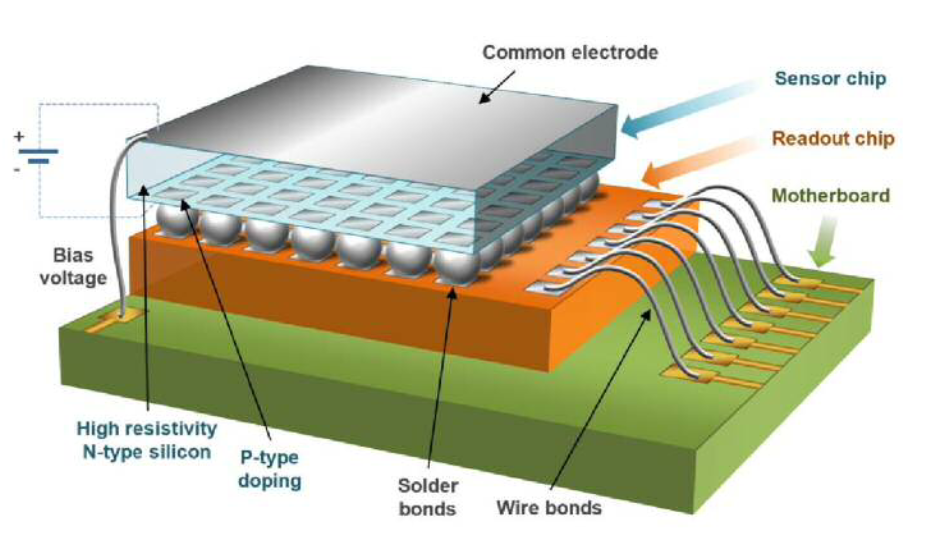
\includegraphics[scale=0.55]{Timepix.png}
 	\caption{Rozložení hybridního pixelového detektoru Timepix \cite{Platkevic}} 
 	\label{fig:Timepix}
 \end{figure}	

\section{Vyčítací zařízení pro pixelové detektory}
\label{Vycitaci zarizeni}
Každý pixelový detektor z rodiny detektorů Timepix \cite{Llopart}, má specifické požadavky pro návrh vyčítacího zařízení. Základními požadavky jakými jsou napájecí napětí detektoru a komunikační rozhraní s detektorem, musí být vždy splněny aby bylo možné spolehlivě komunikovat s pixelovým detektorem. Vyčítacích zařízení existuje celá řada. V této práci, respektive v následujících částech bude popsán návrh miniaturizovaného vyčítacího rozhraní. Pokusím se zde tedy uvést příklady miniaturizovaných zařízení.
\subsection{USB Lite}
Dosud nejmenším vyčítacím zařízení rodiny detektorů Timepix \cite{Llopart}, je zařízení \textit{USB Lite} \cite{usb_lite}, viz. obrázek \ref{fig:usb_lite}. Toto zařízení umožňuje komunikovat s detektorem Medipix 2 \cite{Medpix2}. Rozměry zařízení jsou 60x15 mm. Rychlost vyčítání snímků je 4 fps a spotřeba zařízení je menší než 2 W \cite{usb_lite}.
 \begin{figure}[h!]
	\centering
	\captionsetup{justification=centering}
	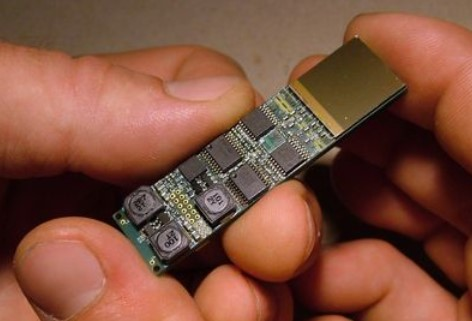
\includegraphics[scale=0.55]{usb_lite.jpg}
	\caption{Vyčítací zařízení \textit{USB lite}} 
	\label{fig:usb_lite}
\end{figure}	

\subsection{MiniPIX SPRINTER}
Vyčítací zařízení MiniPIX SPRINTER je vyvíjeno společností ADVACAM, zařízení je možné vidět na obrázku \ref{fig:sprinter}. Toto zařízení umožňuje komunikovat s detektorem Timepix 2 \cite{tpx2_manual}. Rozměry zařízení jsou 50x21x14 mm. Rychlost vyčítání snímků je 99 \cite{Advacam}.
\begin{figure}[h!]
	\centering
	\captionsetup{justification=centering}
	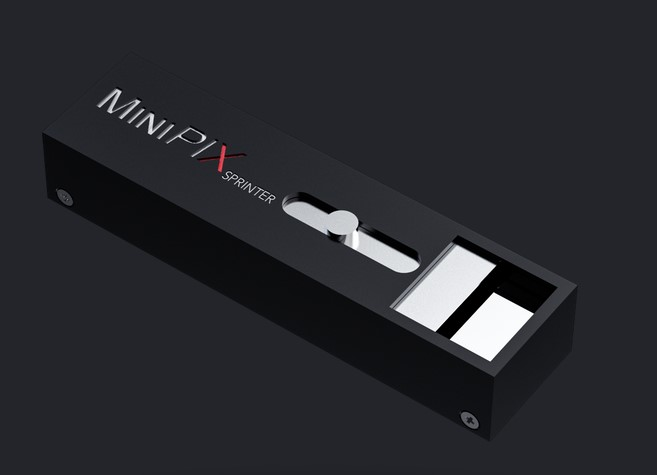
\includegraphics[scale=0.55]{sprinter.jpg}
	\caption{Vyčítací zařízení MiniPIX SPRINTER} 
	\label{fig:sprinter}
\end{figure}	

\subsection{Katherine pro Timepix 2} %katherine zminena protoze modularita
\label{Katherine}
Posledním uvedeným tipem vyčítacího zařízení je zařízení Kathrine pro Timepix 2, které můžete vidět na obrázku \ref{fig:Katherine2}. Toto vyčítací zařízní se od předchozích dvou uvedených liší ve velikosti a maximalní rychlosti komunikace. Zařízení se skládá ze dvou částí. Samotným vyčítacím zařízením, na obrázku \ref{fig:Katherine2} vpravo a takzvaným \textit{chipboardem}, na obrázku \ref{fig:Katherine2} vlevo. Část chipboardu obsahuje detektor Timepix 2 a napájecí zdroje potřebné pro provoz detektoru. Dále jsou ze propojeny signály z konektoru od vyčítacího zařízení po samotný Timepix 2. Výhodou tohoto modulárního zapojení je možnost modifikace chipboardové části, bez nutnosti změn na straně vyčítacího zařízení. Tedy existuje možnost k jednomu vyčítacímu zařízení, připojit různé chipboardy. Parametry samotného vyčítacího zařízení jsou následující. Rozměry 100x80x28 mm, rychlost vyčítaní až 3.2 Gbps \cite{Burian_2020}.
\begin{figure}[h!]
	\centering
	\captionsetup{justification=centering}
	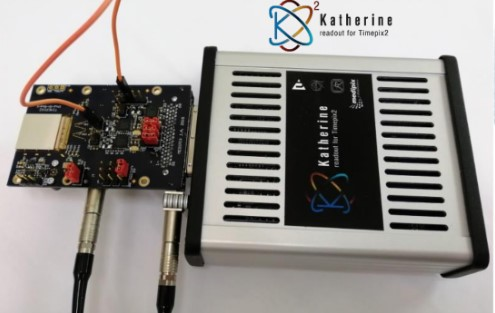
\includegraphics[scale=0.75]{Katherine2.jpg}
	\caption{Vyčítací zařízení Katherine pro Timepix 2 \cite{Burian_2020}} 
	\label{fig:Katherine2}
\end{figure}	

%%%
%%%%%%%%%%%%%%%%%%%%%%%%%%%

\section{Timepix 2}
% v podstatě technická dokumentace Timepix 2, plus konkretni pozadavky pro provoz
\label{Timepix2}
V předchozí části \ref{kap:2.1}, byly popsány obecné vlastnosti pixelových detektoru a základní principy detekce ionizujícího záření. V této kapitole bude detailněji popsán konkrétní detektor, detektor Timepix 2 \cite{tpx2_manual}. Detektor byl vyvinut pod záštitou CERN Medpipix Collaboration \cite{Medpix}. Timepix 2 patří do rodiny detektorů Timepix, kde prvním z rodiny detektorů byl detektor Timepix \cite{Llopart}, následně to popořadě byly detektory Timepix 3 \cite{Timepix3}, Timepix 2 \cite{tpx2_manual}, \cite{Timepix2} a nejnovějším detektorem je Timepix 4 \cite{Timepix4}. Schematické rozložení detektoru Timepix 2 je zobrazeno na obrázku \ref{fig:tpx2_floorplan}. 
\begin{figure}[h!]
	\centering
	\captionsetup{justification=centering}
	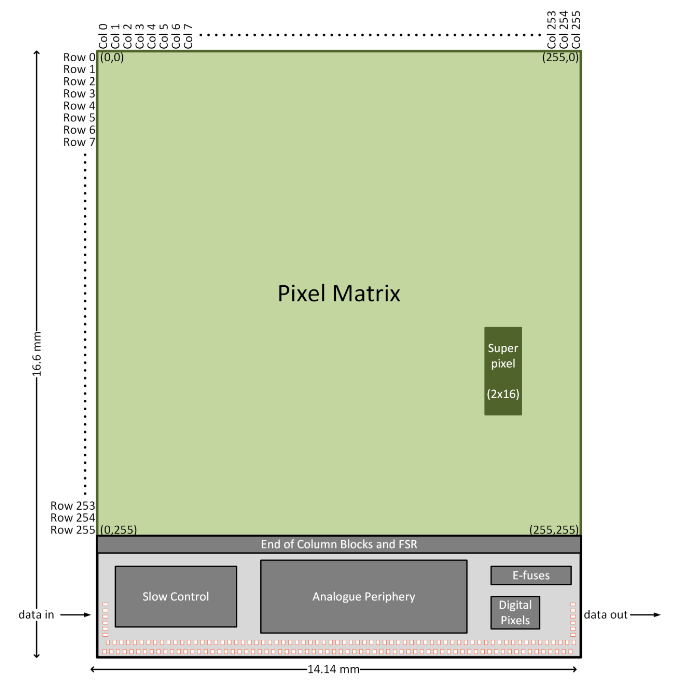
\includegraphics[scale=0.80]{tpx2_floorplan.png}
	\caption{Schematické rozložení detektoru Timepix 2 \cite{tpx2_manual}} 
	\label{fig:tpx2_floorplan}
\end{figure}	

\subsection{Matice pixelů}
Detektro je tvořen maticí 256 x 256 pixelů s roztečí  55 $\mu$$m$. Každý pixel má vlastní analogovou a digitální část, tyto jednotlivé části budou popsány v následujících částech \ref{analog} a \ref{Digitálni cast}. Schematické zobrazení jednoho pixelu detektoru je možné najít na obrázku \ref{fig:tpx2_cell}.
\subsubsection{Analogová část}	 %todo upravit
\label{analog}
Každý pixel z matice 256 x 256 pixelů má vlastní analogovou částí, viz obrázek \ref{fig:tpx2_cell}. Jak bylo zmíněno v kapitole týkající se obecného principu detekce ionizujícího záření za použití pixelových detektorů \ref{kap:2}, pokud částice interaguje na senzorové vrstvě dojde k vytvoření nábojového impulsu. Tento náboj je díky připojenému napětí přitažen k elektrodám. Vytvořený náboj může být charakterizován jako Diracův proudový impuls. Integrací Diracovo proudového impulsu dostaneme celkový generovaný náboj Q. 
\par Tedy analogové zpracování signálů na úrovni jednotlivých pixelů probíhá tak, že diracův proudový impuls vytvořený na senzorové vrstvě je naintegrován do malého kapacitoru $C_{FB}$ z obrázku \ref{fig:tpx2_cell}. Poté na výstupu CSA je v ideálním případě napěťový skok s amplitudou Q/Cf viz. \ref{fig:tpx2_cell}. Výstupní puls je poté porovnán s prahovou úrovní. Nastavením prahové úrovně lze eliminovat zbytkový proud, takzvaný \textit{leakage current}, závěrného směru polovodičové struktury, který zde vznikl kvůli připojenému vysokému napětí. Pokud je signál větší než daná nastavená úroveň, je inkrementován digitální čítač \cite{Llopart}. Každý diskriminátor obsahuje 5-bitový DAC převodník. Tento 5 bitový DAC převodník umožňuje nastavit úroveň detekovatelného signálu pro každý pixel individuálně a tím eliminovat šum způsobený zbytkovým proudem polovodičové struktury.
\par Pokud není povolena funkce adaptivního zesílení signálu, ve zpětné vazbě CSA z obrázku \ref{fig:tpx2_cell} je fixní hodnota kondenzátoru $C_{FB}$. Tedy dochází k rovnoměrnému zesílení vstupního signálu, bez ohledu na velikosti generovaného náboje. 
\par Pokud je povolen režim adaptivního zesílení zpětné vazba CSA je tvořena kondenzátorem $C_{FB}$ paraelně s kapacitou MOS tranzistoru. Zesílení vstupního signálu je vysoké pro vstupní signály s malou amplitudou a nízké pro signály s vysokou amplitudou, více viz. \cite{MOS}.
\begin{figure}[h!]
	\centering
	\captionsetup{justification=centering}
	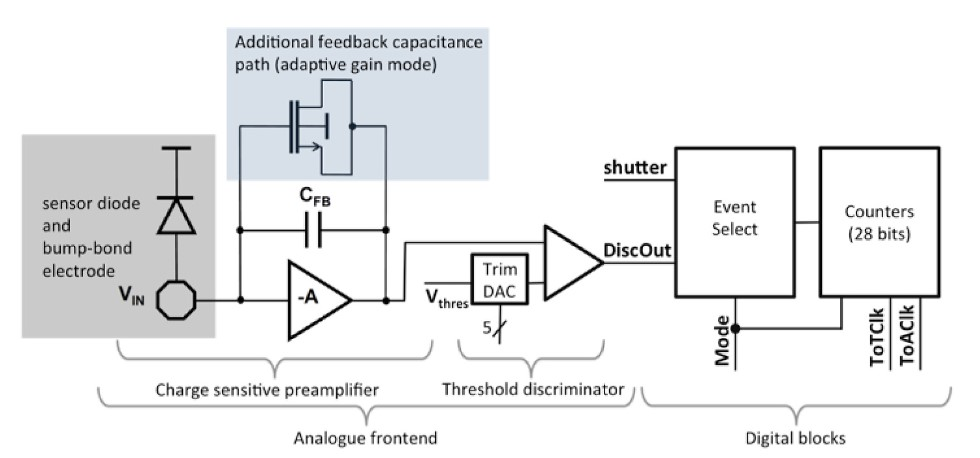
\includegraphics[scale=0.70]{tpx2_cel.jpg}
	\caption{Uspořádání jednoho pixelu \cite{Timepix2}}
	\label{fig:tpx2_cell}
\end{figure}

\subsubsection{Digitální část}
\label{Digitálni cast}
Zobrazení digitální části jednotlivých pixelů, je možné vidět na obrázku \ref{fig:tpx2_cell}. Každý pixel obsahuje digitální 28 bitové čítače. Konkrétně se jedná o čtyři digitální čítače typu LSFR. V případě Timepix 2 každý pixel obsahuje dva 10-bitové (označení: A,B) a dva 4-bitové (označení: C,D) čítače. Tedy například 14-bitový čítač lze jednoduše vytvořit kombinací 10-bitového a 4-bitového čítače. Kvůli použití lineárně posuvného čítače LSFR, každý n-bitový čítač generuje $2^n$ pseoudonáhodných čísel. Odpovídající dekódovaná hodnota pseudonáhodného čísla lze pro příklad čtrnácti bitového čítače vidět v rovnici \ref{eq:1}. Digitální čítače, respektive části jednotlivých čítačů, mohou pracovat v různých módech, které budou následně popsány.

\begin{equation}
	14-bit = (hodnota_{4-bit} \cross 2^{10}) + hodnota_{10-bit}
	\label{eq:1}
\end{equation}

Jak bylo zmíněno výše. Každý z digitálních čítačů může být nakonfigurován do jiného módu. Pro Timepix 2 jsou to následující módy \ref{fig:modes}. 
\begin{itemize}
	\item \textbf{Time over Threshold} (ToT): Čítač je inkrementován při každém hodinovým pulsu, kdy je signál nad nastavenou prahovou úrovní
	\item \textbf{Time of Arrival} (ToA): Čítač je inkrementován při každém hodinovým pulsu, kdy signál překročí nastavenou úroveň a inkrementuje se až do konce akvizice.
	\item \textbf{Coutnig mode}: Čítač je inkrementován pokud pokud došlo k překročení nastavené prahové úrovně detekce.
\end{itemize}
\begin{figure}[h!]
	\centering
	\captionsetup{justification=centering}
	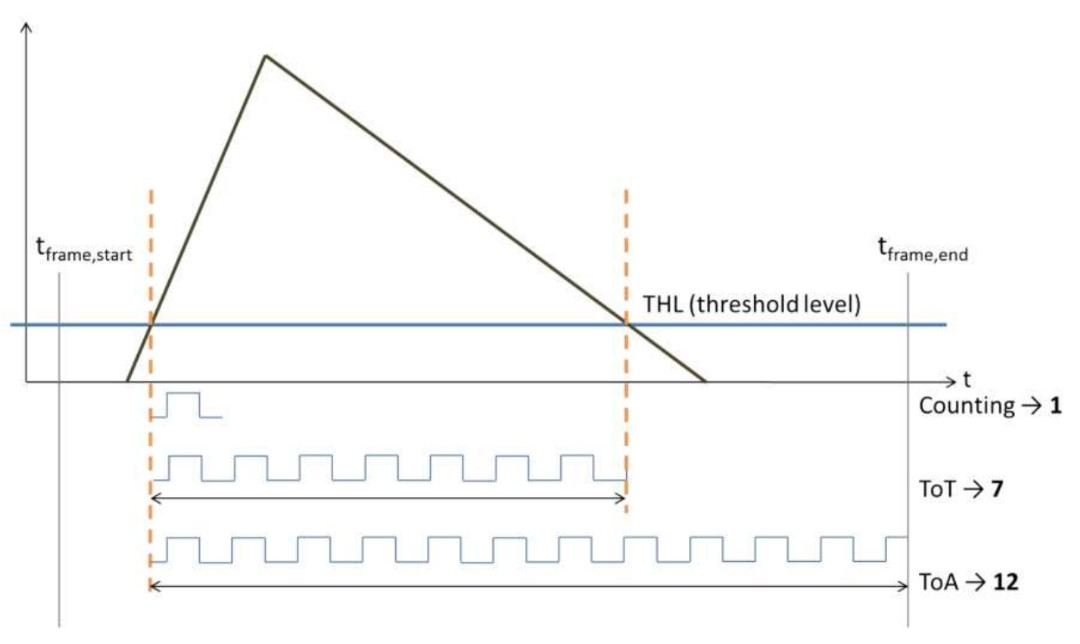
\includegraphics[scale=0.45]{modes.jpg}
	\caption{Digitální módy Timepix 2 \cite{Manek}} 
	\label{fig:modes}
\end{figure}	
\par Celkem lze použít 8 digitálních módu. Každý jednotlivý mód určuje, jaká informace bude v jakém čítači uložena. Například při použití digitálního módu 1 je do 10 bitového čítače ukládána informace ToT a do 18 bitového čítače je ukládána informace ToA. Více o jednotlivých digitálních módech Timepix 2 lze dohledat v technické dokumentaci \cite{tpx2_manual}.

\par Výhodou detektoru Timepix 2 je, že pro použití módu ToT a ToA lze použít rozdílný zdroj hodinového signálu pro měření.

\par Digitální čítače mimo výše popsaných digitálních módů můžou pracovat buď v simultánním, nebo kontinuálním režimu. Simultánní režim znamená, že naměřená data musí být vyčtena z 28 bitového digitálního čítače, kdy při vyčítání není možné měřit příchozí ionizující záření. Doba kdy detektor nemůže měřit příchozí záření vlivem samotného vyčítaní dat se nazývá mrtvá doba detektoru. Pro Timepix 2 při použití sériového komunikačního rozhraní s frekvencí hodinového signálu 100 MHz je tato doba 2.6 ms. Druhým režimem je režim kontinuální. Výhodou kontinuálního režimu je, že zde je nulová mrtvá doba. Princip činnosti je zjednodušeně, že dva digitální čítače jsou nastaveny na stejnou velikost, přičemž do jednoho z čítačů se ukládá informace, dle nastaveného měřícího módu. Tento čítač je zřetězení s druhým čítačem s identickou velikostí, ze kterého se pouze vyčítá. 

\par Příkladem použití digitálních módů může být způsob měření energie, kterou interagující částice zanechala v senzoru. Tuto energii můžeme zjistit pokud vybereme digitální mód, při kterém se do některého z čítačů ukládá informace z ToT měření. Počet zaznamenaných hodinových taktů odpovídá času, po který hodnota analogového napětí signálu byla nad nastavenou detekovatelnou úrovní. Více o způsobu měření energie, kterou částice zanechala v detektoru lze dohledat například v \cite{JAKUBEK2011S262}.

%TODO zminit ze countery mouhu ruzne kombinovat a zaroven jejich mody. PLUS zminit maskovani pixelu -> spotreba

\subsection{Komunikační rozhraní}
\label{Komunikacni rozhrani}
Timepix 2 umožňuje komunikaci po paraelním nebo sériovém datovém rozhraní. Pro paraelní komunikaci je možno využít 32 paraelních vodičů. Paraelní brána dosahuje násobně vyšších přenosových rychlostí, záleží na počtu použitých paraelních vodičů, než sériové rozhraní, viz. obrázek \ref{fig:rychlosti}. Pro dosažením takovýchto rychlostí, respektive paraelního zpracování dat je zapotřebí na straně vyčítací elektroniky použít velmi rychlé rozhraní, například FPGA.  
\par Sériová komunikace probíhá po diferenciálních datových párech. Konkrétně se jedná o komunikační specifikaci SLVS \cite{SLVS}. Napěťové úrovně této specifikace lze najít na obrázku \ref{fig:SLVS_LVDS}. Jak lze z obrázku \ref{fig:SLVS_LVDS} vidět, specifikace SLVS je analogická ke komunikační specifikaci LVDS \cite{LVDS}. Maximální rychlost komunikačních hodin pro použití sériového rozhraní je dle manuálu Timepix 2 \cite{tpx2_manual} 100 Mhz. Z uvedených parametrů týkající se maximální rychlosti komunikace, lze na straně vyčítacího zařízení navrhnout například použití mikroprocesoru. Hlavní nevýhodou sériové komunikace je maximální vyčítací rychlost, která je násobně nižší než při použití komunikace paraelní \ref{fig:rychlosti}. Naopak výhody sériové komunikace jsou především jednoduchost implementace a také teoreticky nižší spotřeba vyčítacího zařízení detektoru.
\begin{figure}[h!]
	\centering
	\captionsetup{justification=centering}
	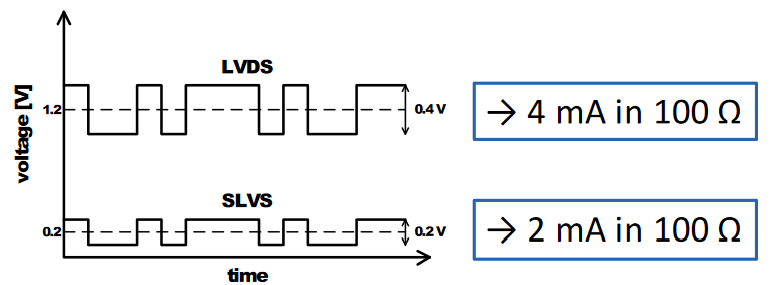
\includegraphics[scale=0.55]{SLVS_LVDS.png}
	\caption{SLVS specifikace \cite{SLVS}} 
	\label{fig:SLVS_LVDS}
\end{figure}	

%TODO MCLOCK????
\subsection{Technické specifikace} %napáječky, kom. rozhraní, prikazy atd.., VN, hodiny pro měření, I/O piny
\label{Technicka specifikace}
Timepix 2 je rozdělen do 256 x 256 pixelů. Rozteč mezi jednotlivými pixely je 55 $\mu$$m$. Celkově rozměry Timepix 2 jsou 16.6 x 14.14 mm. Vyčítací část detektoru tvoří ASCI chip navržen ve 130 nm CMOS technologii. Samotná výroba ASIC je zajišťována jedním z předních výrobců chipů, firmou TSMC \cite{TSMC} na Taiwanu. Všechny technické informace, nebude-li uvedeno jinak jsou čerpány z manuálu k detektoru Timepix 2. \cite{tpx2_manual}.

\subsubsection{Napájení}	
Timepix 2 ke své činnosti potřebuj celkem 3 napájení viz. tabulka \ref{tab:tpx2_napajeni}. Napájení VDD slouží pro napájení digitální části jádra Timepix2 a VDDA slouží k napájení analogové části jádra Timepix  2. Napájení VDDIO slouží k napájení vstupních/výstupních bran. Posledním uvedeným napájení v tabulce \ref{tab:tpx2_napajeni} je napájení VDD33. Toto napájení je potřeba přepínat, podle potřebné funkcionality detektoru. Pokud chceme z Timepix 2 vyčíst CHIP ID, musíme na pin VDD33 aplikovat napájecí napětí 2.5 V. Při ostatní činnosti detektoru, je požadováno aby napětí označené VDD33 bylo 1.2 V. 
\begin{table}[h!]
	\centering
	\begin{tabular}{ |P{3cm}||P{5cm}|  }
		\hline
		\multicolumn{2}{|c|}{Napájecí úrovně Timepix 2} \\
		\hline
		Název pinu& Hodnota napájecího napětí [V] \\ \hline \hline 
		VDDIO & 2.5 \\ \hline		
		VDD & 1.2 \\ \hline 		 
		VDDA & 1.2 \\ \hline
		VDD33 & 2.5 (1.2)\\ \hline
	\end{tabular}
	\caption{Napájecí úrovně Timepix 2}
	\label{tab:tpx2_napajeni}
\end{table}
\par Speciální kategorií napájení je napájení pro zajištění vysokého napětí, které je připojeno na senzorovou vrstvu. Toto napětí zajistí vyprázdnění oblasti v polovodičové struktuře. Požadavky na parametry vysokého napětí záleží na typu a tloušťce senzorové vrstvy. Nejčastěji používaným materiálem senzorové vrstvy je křemík, ovšem záleží na příkladu použití detektoru. Uvedu-li příklad vysokého napětí, které bylo použito pro testování Timepix 2 s křemíkovou senzorovou vrstvou o tloušťce 500 $\mu$m dle \cite{Timepix2_500um} bylo 100 V. Další příklady velikosti vysokého napětí používaných pro různé senzorové vrstvy lze najít v odkazech \cite{Timepix_500um_Pospisil}, \cite{Timepix_500um_Huston}. Důležitou vlastností vysokonapěťových zdrojů je možnost nastavení výstupního vysokého napětí v určitém rozsahu.   

\subsubsection{Spotřeba}	
Celková spotřeba Timepix 2 dle \cite{Timepix2} při zapnutí všech pixelů a frekvenci datových hodin $f_{clock}$ = Mhz je nižší než 900 mW. Přičemž spotřeba jednoho pixelu je 5 $z\mu$A.
\par Timepix 2 disponuje možnostmi, jak celkovou spotřebu detektoru snížit. Ke celkovému snížení spotřeby slouží funkcionalita, která umožňuje zamaskovat pixely, které nebudou dále použity pro ukládání informace z měření. Dojde k téměř kompletnímu vypnutí vybraných pixelů. Z výše uvedené spotřeby pro jeden pixel, se pro vybraný pixel, který má být vypnut, dostáváme na spotřebu okolo jednotek nA na pixel.

\subsubsection{Rychlost komunikace}
V části \ref{Komunikacni rozhrani}, byly popsány možnosti využití paraelního, či sériového rozhraní pro komunikaci s Timepix 2. Dobra pro vyčtení celé matice pixelů pro oba typy rozhraní lze vidět na obrázku \ref{fig:rychlosti}. 
\begin{figure}[h!]
	\centering
	\captionsetup{justification=centering}
	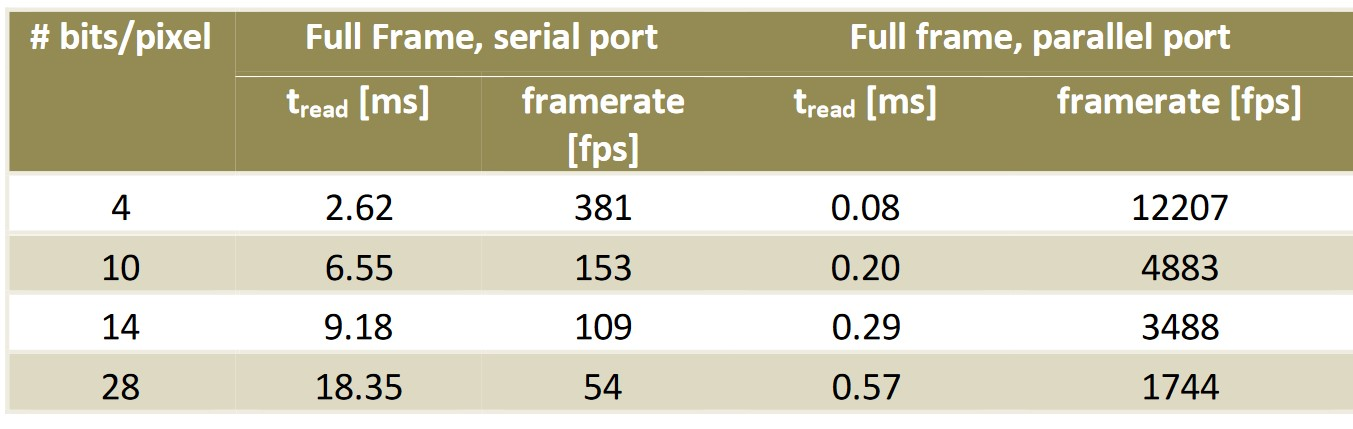
\includegraphics[scale=0.65]{rychlosti.jpg}
	\caption{Vyčítací rychlosti snímků z Timepix2. Frekvence hodin $f_{clock}$ = 100 MHz \cite{Timepix2}} 
	\label{fig:rychlosti}
\end{figure}	

Poslední možností vyčítání dat z Timepix 2 je použití ZCS módu. Tento mód lze použít při vyčítání dat přes sériové rozhraní. Na obrázku \ref{fig:rychlosti}, lze vidět, že tento mód je rychlejší než použití sériového rozhraní při vyčítání celých snímku. Při použití ZCS módu nejprve detektor odešle 256 bitů, které odpovídají jednotlivým sloupcům detektoru. V těchto 256 bitech je uložena informace o tom, zda-li došlo v příslušném sloupci k detekci ionizujícího záření. Pokud ano, bude sloupec nastaven na logickou hodnotu 1. V opačném případě zůstává hodnota sloupce v logické nule. Po obdržení 256 bitů je přijato tolik dat, kolik sloupců bylo zasaženo. Avšak minimálně bude vždy posláno 16 sloupců i kdyby nebyla detekována žádná částice. Velikost poslaných dat za použití ZCS módu je tedy vždy závislá na aktivitě ionizujícího záření a s tím i spojená vyčítací rychlost. Pokud by byly aktivovány všechny pixely, bude rychlost ZCS módu nanejvýše stejně rychlá, jako při vyčtení celého snímku. Na obrázku \ref{fig:rychlosti} je pro ZCS mód uvažováno vyčtení 16 sloupců matice.



\subsubsection{Rozhraní pro připojení Timepix 2 k desce plošných spojů}	% TODO nazev
Připojení Timepix 2 k desce plošných spojů je nejčastěji realizováno pomocí technologie \textit{wire bonding}. Timepix 2 má celkem 152 pinů pro přichycení wire bondů. Rozložení pinů je zobrazeno na obrázku \ref{fig:tpx2_floorplan} ve spodní části. Rozteč mezi jednotlivými plošky je 108 $\mu$m.

Dalším možným způsobem připojení Timepix 2 k desce plošných spojů je pomocí technologie zvané TSV. Respektive pomocí této technologie je možné signály vyvést ze zadní strany Timepix 2 k pájecím ploškám. Vznikne tím tak uspořádání, známe z technologie výroby pouzder BGA elektronických součástek. 
\par Běžnější způsob připojení Timepix 2 k desce plošných spojů je pomocí wire bondů. Použití wire bondů i technologie BGA je možné vidět na obrázku \ref{fig:bga}. Výhodou oproti technologii wire bondů je lepší praktické zacházení, díky absenci tenkých wire bondů, které jsou velmi náchylné na mechanické poškození. Další výhodou je poté technologicky méně náročné připojení detektoru. Avšak nevýhodou této technologie je vystavení chipu vysoké teplotě při pájení.
\begin{figure}[h!]
	\centering
	\captionsetup{justification=centering}
	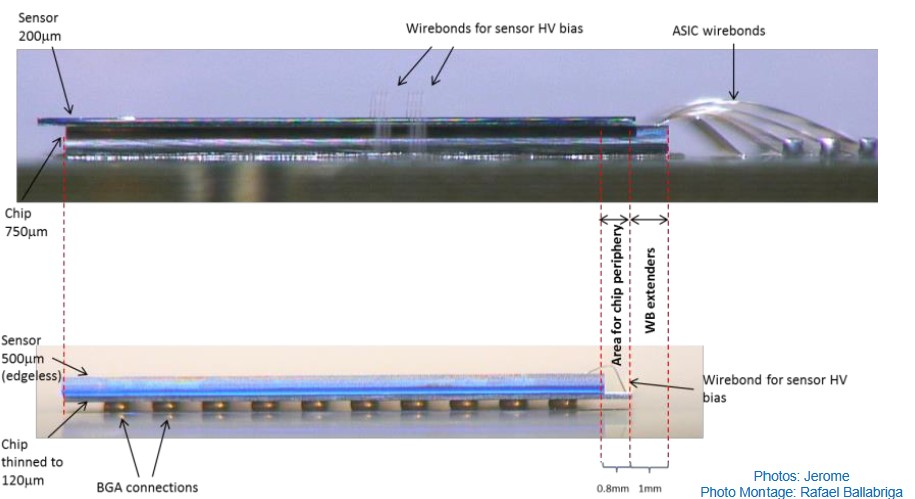
\includegraphics[scale=0.55]{bga.jpg}
	\caption{Připojení detektoru Timepix 2 k desce plošných spojů \cite{TSV}} 
	\label{fig:bga}
\end{figure}	









